	\documentclass{libs/ufc_format}
\usepackage{amsmath, tikz, graphicx}
\usetikzlibrary{trees,shapes, calc, external, fit, arrows,decorations,decorations.pathreplacing,patterns, automata, positioning, arrows.meta}

\newcommand{\live}{\ensuremath{L}\xspace}
\newcommand{\evict}{\ensuremath{\mathcal{V}}\xspace}
\newcommand{\taskset}{\ensuremath{\mathbb{T}}\xspace}
\newcommand{\inputs}{\ensuremath{\mathcal{D}}\xspace}
\newcommand{\nbloads}{\ensuremath{\mathit{\mathit{\#Loads}}}\xspace}
\newcommand{\starpu}{\textsc{StarPU}\xspace}
\newcommand{\threeinputs}{\textbf{3inputs}\xspace}
\newcommand{\OPTI}{\textbf{OPTI}\xspace}
\newcommand{\GPU}[1]{\ensuremath{\mathrm{GPU}_{#1}}\xspace}
\newcommand{\Dtouse}[1]{\ensuremath{\mathit{dataNotInMem}_{#1}}\xspace}
\newcommand{\plannedTasks}[1]{\ensuremath{\mathit{plannedTasks}_{#1}}\xspace}
\newcommand{\Dopt}{\ensuremath{D_{\mathit{opt}}}\xspace}
\newcommand{\Treturned}{\ensuremath{T}\xspace}
\newcommand{\pulledTasks}[1]{\ensuremath{\mathit{taskBuffer}_{#1}}\xspace}
%%%%%%%%%%%%%%%%%%%%%%%%%%%%%%%%%%%%%%%%%%%%%%%%%%%%%%%%%%%%%%%%%%%%%%%%%%%%%%%%%%%

% For the arrows in circle
\setcounter{tocdepth}{1}
\usetikzlibrary{decorations.text}
\newcommand*{\mytextstyle}{\sffamily\small\bfseries\color{black!85}}
\newcommand{\arcarrow}[8]{%
% inner radius, middle radius, outer radius, start angle,
% end angle, tip protusion angle, options, text
  \pgfmathsetmacro{\rin}{#1}
  \pgfmathsetmacro{\rmid}{#2}
  \pgfmathsetmacro{\rout}{#3}
  \pgfmathsetmacro{\astart}{#4}
  \pgfmathsetmacro{\aend}{#5}
  \pgfmathsetmacro{\atip}{#6}
  \fill[#7] (\astart:\rin) arc (\astart:\aend:\rin)
       -- (\aend+\atip:\rmid) -- (\aend:\rout) arc (\aend:\astart:\rout)
       -- (\astart+\atip:\rmid) -- cycle;
  \path[font = \sffamily, decoration = {text along path, text = {|\mytextstyle|#8},
    text align = {align = center}, raise = -0.5ex}, decorate]
    (\astart+\atip:\rmid) arc (\astart+\atip:\aend+\atip:\rmid);
}

\newcommand{\nologo}{\setbeamertemplate{logo}{}} % command to set the logo to nothing

% Inserting the preamble file with the packages
%%%%%%%%%%%%%%%%%%%%%%%%%%%%%%%%%%%%%%%%%%%%%%%%%%%%%%%%%%%%%%%%%%%%%
%% This file contains the packages that can be used in the beamer. %%
%%%%%%%%%%%%%%%%%%%%%%%%%%%%%%%%%%%%%%%%%%%%%%%%%%%%%%%%%%%%%%%%%%%%%
% Package to fonts family
\usepackage[T1]{fontenc}
% Package to accentuation
\usepackage[utf8]{inputenc}
% Package to Portuguese language
\usepackage[english]{babel}
% Package to Figures
\usepackage{graphicx}
% Package to the colors
\usepackage{color}
% Package to the colors
\usepackage{xcolor}
% Packages to math symbols and expressions
\usepackage{amsfonts, amssymb, amsmath}
% Package to multiple lines and columns in table
\usepackage{multirow, array} 
% Package to create pseudo-code
% For more detail of this package: http://linorg.usp.br/CTAN/macros/latex/contrib/algorithm2e/doc/algorithm2e.pdf
\usepackage{algorithm2e}
% Package to insert code
\usepackage{listings} 
\usepackage{keyval}
% Package to justify text
\usepackage[document]{ragged2e}
% Package to manage the bibliography
\usepackage[backend=biber, style=numeric, sorting=none]{biblatex}
% Package to facilities quotations
\usepackage{csquotes}
% Package to use multicols
\usepackage{multicol}
% Subfigures
\usepackage{subcaption}
\usepackage{marvosym} % \MVRIGHTarrow

% Inserting the references file
\bibliography{../ref_cadre.bib}

% Title
\title[Memory-Aware Scheduling]{\huge\textbf{Memory-Aware Scheduling of Tasks Sharing Data on Multiple GPUs with Dynamic Runtime Systems}}
% Subtitle
\subtitle{36th IEEE International Parallel \& Distributed Processing Symposium}
% Author of the presentation
\author{\underline{Maxime GONTHIER} - Loris MARCHAL - Samuel THIBAULT}
% Institute's Name
\institute[UFC]{
    % email for contact
    %~ \normalsize{Loris MARCHAL - Samuel THIBAULT}
    \normalsize{\email{maxime.gonthier@ens-lyon.fr}}
    \newline
    % Department Name
    \department{LIP - ROMA - LaBRI - STORM}
    \newline
    
\includegraphics[scale=0.05]{Images/solahris+inria.png}%
    % university name
    %~ \univ
}
%~ \titlegraphic{
\includegraphics[scale=0.5]{Images/logo_solharis_full2.png}}

% date of the presentation
% \date{\today}
%~ \usepackage{datetime}
%~ \newdate{date}{01}{06}{2022}
%~ \date{\displaydate{date}}


%%%%%%%%%%%%%%%%%%%%%%%%%%%%%%%%%%%%%%%%%%%%%%%%%%%%%%%%%%%%%%%%%%%%%%%%%%%%%%%%%%
%% Start Document of the Presentation                                           %%               
%%%%%%%%%%%%%%%%%%%%%%%%%%%%%%%%%%%%%%%%%%%%%%%%%%%%%%%%%%%%%%%%%%%%%%%%%%%%%%%%%%
\begin{document}
% insert the code style
%%%%%%%%%%%%%%%%%%%%%%%%%%%%%%%%%%%%%%%%%%%%%%%%%%%%%%%%%%%%%%%%%%%%%%%%%%%%%%%%%%%
%% This file contains the style of the codes show in slides.                     %%
%% The package used is listings, but it possible to used others.                 %%
%%%%%%%%%%%%%%%%%%%%%%%%%%%%%%%%%%%%%%%%%%%%%%%%%%%%%%%%%%%%%%%%%%%%%%%%%%%%%%%%%%%

% color used in the code style
\definecolor{codegreen}{rgb}{0,0.6,0}
\definecolor{codegray}{rgb}{0.5,0.5,0.5}
\definecolor{codepurple}{rgb}{0.58,0,0.82}
\definecolor{codebackground}{rgb}{0.95,0.95,0.92}

% style of the code!
\lstdefinestyle{codestyle}{
    backgroundcolor=\color{codebackground},   
    commentstyle=\color{codegreen},
    keywordstyle=\color{magenta},
    numberstyle=\tiny\color{codegray},
    stringstyle=\color{codepurple},
    basicstyle=\ttfamily\footnotesize,
    frame=single,
    breakatwhitespace=false,         
    breaklines=true,                 
    captionpos=b,                    
    keepspaces=true,                 
    numbers=left,                    
    numbersep=5pt,                  
    showspaces=false,                
    showstringspaces=false,
    showtabs=false,                  
    tabsize=2,
    title=\lstname 
}

\lstset{style=codestyle}


%% ---------------------------------------------------------------------------
\begin{frame}{}
    \maketitle
\end{frame}

%~ %% ---------------------------------------------------------------------------
%~ \begin{frame}{Summary}
    %~ \begin{multicols}{2}
        %~ \tableofcontents
    %~ \end{multicols}
%~ \end{frame}

%% ---------------------------------------------------------------------------
\section{Motivation and formalization}
\begin{frame}{Motivation: Extract peak performances from GPUs}
	\vspace{-0.8cm}
	\hspace{-0.9cm}
	\begin{figure}[tb]
		\definecolor{green}{RGB}{70, 220, 70}
		\definecolor{orangegray}{RGB}{245, 191, 169}
		\centering
		\scalebox{0.73}{
		\begin{tikzpicture}[thick]
			\def\x{1.2}
			\def\y{1.5}
			\draw[color=black, fill=orangegray] (0*\x, 2*\y) rectangle (2*\x, 3*\y)  node[midway] {$\GPU{1}$ memory}; 
			\draw[color=black, fill=orangegray] (3*\x, 2*\y) rectangle (5*\x, 3*\y)  node[midway] {$\GPU{2}$ memory}; 
			\draw[color=black, fill=orangegray] (6*\x, 2*\y) rectangle (8*\x, 3*\y)  node[midway] {$\GPU{3}$ memory}; 
			\draw[color=black, fill=orangegray] (9*\x, 2*\y) rectangle (11*\x, 3*\y)  node[midway] {$\GPU{4}$ memory};
			\draw[color=black, fill=green] (0*\x, 0*\y) rectangle (11*\x, 1*\y) node[midway] {CPU memory of infinite size}; 
			\path[ultra thick] (5.5*\x,1*\y) edge (5.5*\x,1.4*\y); 
			\path[ultra thick] (1*\x,1.4*\y) edge node[midway, above] {PCI Express bus} (10*\x,1.4*\y); 
			\path[ultra thick] (1*\x,1.4*\y) edge (1*\x,2*\y); 
			\path[ultra thick] (4*\x,1.4*\y) edge (4*\x,2*\y);
			\path[ultra thick] (7*\x,1.4*\y) edge (7*\x,2*\y); 
			\path[ultra thick] (10*\x,1.4*\y) edge (10*\x,2*\y); 
			% Arrow 1
			\node at (-0.4, 0) (n1){};
			\node(n2)[above=3.5cm of n1]{};
			% this path will place/draw a node call (text)
			\scalebox{1.3}{\path (n1) -- node[sloped] (text) {Loading data} (n2);
			% Now draw arrows. This way it will be like you want.
			\draw[ultra thick][->] (n1)--(text)--(n2);}
			% Arrow 2
			\node at (10.5, 0) (n1){};
			\node(n2)[above=3.5cm of n1]{};
			\scalebox{1.3}{\path (n1) -- node[sloped] (text) {Evicting data} (n2);
			\draw[ultra thick][->] (n2)--(text)--(n1);}
		\end{tikzpicture}
		}
		\label{fig.topo}
	\end{figure}
	\successbox{GPUs are fast but have a limited memory}
	\successbox{Share the same PCI bus with limited bandwidth}
\end{frame}

%% ---------------------------------------------------------------------------
%~ \section{Formalization of the problem}
\subsection{Framework}
\begin{frame}{Framework: An example with 2D grid dependencies}
\begin{figure}[tb]
\definecolor{blue}{rgb}{0.38, 0.51, 0.71} %glaucous, 97,130,181, #6182B5
\definecolor{darkblue}{RGB}{17, 42, 60} % 112A3C
\definecolor{red}{RGB}{175, 49, 39} % AF3127
\definecolor{otherred}{RGB}{171,78,78}
\definecolor{orange}{RGB}{237, 126, 75} 
\definecolor{green}{RGB}{104, 174, 89} 
\definecolor{palegreen}{RGB}{197, 184, 104} 
\definecolor{yellow}{RGB}{250, 199, 70} % FAC764
\definecolor{brokenwhite}{RGB}{218, 192, 166} % DAC0A6
\definecolor{brokengrey}{rgb}{0.77, 0.76, 0.82} % {196,194,209}, C4C2D1
  \scalebox{0.672}{
  \begin{tikzpicture}[
    semithick,
    ]
    \tikzstyle{every state}=[ draw = black, thick, fill = white, minimum size = 8mm ]
    \draw[fill=lightgray,draw=none,rounded corners=10pt] (-0.5,0.5)    rectangle (1.8,-1.8);
    \draw[fill=lightgray,draw=none,rounded corners=10pt] (-0.5,-3.1)    rectangle (3.1,-2.2); 
    \draw[fill=lightgray,draw=none,rounded corners=10pt] (2.2,-3.1)    rectangle (3.1,0.5); 
    \node[state] (T1) at (0,0){$T_1$};
    \node[state] (T2) [right=0.5cm of T1] {$T_2$}; 
    \node[state] (T3) [right=0.5cm of T2] {$T_3$}; 
    \node[state] (T4) [below=0.5cm of T1] {$T_4$};
    \node[state] (T5) [right=0.5cm of T4] {$T_5$}; 
    \node[state] (T6) [right=0.5cm of T5] {$T_6$}; 
    \node[state] (T7) [below=0.5cm of T4] {$T_7$};
    \node[state] (T8) [right=0.5cm of T7] {$T_8$}; 
    \node[state] (T9) [right=0.5cm of T8] {$T_9$}; 

    \node[state, fill=yellow] (D1) [above=0.9cm of T1] {$D_1$}; 
    \node[state, fill=orange] (D2) [above=0.9cm of T2] {$D_2$}; 
    \node[state, fill=red!80] (D3) [above=0.9cm of T3] {$D_3$}; 
    \node[state, fill=blue] (D4) [left=0.9cm of T1] {$D_4$}; 
    \node[state, fill=green] (D5) [left=0.9cm of T4] {$D_5$}; 
    \node[state, fill=palegreen] (D6) [left=0.9cm of T7] {$D_6$}; 
    \draw (T1) to [bend right] (D1); 
    \draw (T2) to [bend right] (D2); 
    \draw (T3) to [bend right] (D3); 
    \draw (T1) to [bend left] (D4); 
    \draw (T4) to [bend left] (D5); 
    \draw (T7) to [bend left] (D6); 
[    \draw (T4) to [bend right] (D1); 
    \draw (T5) to [bend right] (D2); 
    \draw (T6) to [bend right] (D3);
    \draw (T7) to [bend right] (D1); 
    \draw (T8) to [bend right] (D2); 
    \draw (T9) to [bend right] (D3); 
    \draw (T2) to [bend left] (D4); 
    \draw (T5) to [bend left] (D5); 
    \draw (T8) to [bend left] (D6); 
    \draw (T3) to [bend left] (D4); 
    \draw (T6) to [bend left] (D5); 
    \draw (T9) to [bend left] (D6); 
  \end{tikzpicture}%
}
\scalebox{0.672}{
\begin{tikzpicture}[semithick, > = {Stealth[scale=1.25]}, shorten > = 1pt,]
    \def\x{1}
    \def\y{0.6}
    \draw[color=black] (0*\x+0.02, 0.4) rectangle (1*\x-0.02, -0.1) node[midway] {$T_1$}; 
    \draw[color=black] (1*\x+0.02, 0.4) rectangle (2*\x-0.02, -0.1) node[midway] {$T_2$}; 
    \draw[color=black] (2*\x+0.02, 0.4) rectangle (3*\x-0.02, -0.1) node[midway] {$T_5$}; 
    \draw[color=black] (3*\x+0.02, 0.4) rectangle (4*\x-0.02, -0.1) node[midway] {$T_4$};   
    \draw[color=black, fill=blue] (0*\x, 2*\y) rectangle (2*\x, 3*\y) node[midway] {$D_4$};
    \draw[color=black, fill=green] (2*\x, 2*\y) rectangle (4*\x, 3*\y) node[midway] {$D_5$};
    \draw[color=black, fill=yellow] (0*\x, 1*\y) rectangle (1*\x, 2*\y)  node[midway] {$D_1$}; 
    \draw[color=black, fill=orange] (1*\x, 1*\y) rectangle (3*\x, 2*\y)  node[midway] {$D_2$}; 
    \draw[color=black, fill=yellow] (3*\x, 1*\y) rectangle (4*\x, 2*\y)  node[midway] {$D_1$}; 
    \draw (4*\x,2*\y) node[right]{\it \small data in memory};
    \draw (4,0.15) node[right] {\it \small tasks being processed };
    \draw[thick, decoration={brace,amplitude=5pt},decorate] (-0.1,-0.1) -- node[left=4pt] {\GPU{1}} (-0.1, 3*\y); 
    \def\yshift{2.5}
    \draw[color=black, fill=blue] (0*\x, 1*\y+\yshift) rectangle (1*\x, 2*\y+\yshift)  node[midway] {$D_4$}; 
    \draw[color=black, fill=green] (1*\x, 1*\y+\yshift) rectangle (2*\x, 2*\y+\yshift)  node[midway] {$D_5$}; 
    \draw[color=black, fill=palegreen] (2*\x, 1*\y+\yshift) rectangle (5*\x, 2*\y+\yshift)  node[midway] {$D_6$}; 
    \draw[color=black, fill=red!80] (0*\x, 2*\y+\yshift) rectangle (3*\x, 3*\y+\yshift)  node[midway] {$D_3$}; 
    \draw[color=black, fill=orange] (3*\x, 2*\y+\yshift) rectangle (4*\x, 3*\y+\yshift)  node[midway] {$D_2$}; 
    \draw[color=black, fill=yellow] (4*\x, 2*\y+\yshift) rectangle (5*\x, 3*\y+\yshift)  node[midway] {$D_1$}; 
    \draw[color=black] (0*\x+0.02, 0.4+\yshift) rectangle (1*\x-0.02, -0.1+\yshift) node[midway] {$T_3$}; 
    \draw[color=black] (1*\x+0.02, 0.4+\yshift) rectangle (2*\x-0.02, -0.1+\yshift) node[midway] {$T_6$}; 
    \draw[color=black] (2*\x+0.02, 0.4+\yshift) rectangle (3*\x-0.02, -0.1+\yshift) node[midway] {$T_9$}; 
    \draw[color=black] (3*\x+0.02, 0.4+\yshift) rectangle (4*\x-0.02, -0.1+\yshift) node[midway] {$T_8$}; 
    \draw[color=black] (4*\x+0.02, 0.4+\yshift) rectangle (5*\x-0.02, -0.1+\yshift) node[midway] {$T_7$}; 
    \draw (5*\x,2*\y+\yshift) node[right]{\it \small data in memory};
    \draw (5,0.15+\yshift) node[right] {\it \small tasks being processed};
    \draw[thick, decoration={brace,amplitude=5pt},decorate] (-0.1,-0.1+\yshift) -- node[left=4pt] {\GPU{2}} (-0.1, 3*\y+\yshift); 
    \path[->, thick] (0*\x,-0.5) edge node[midway, below] {time} (7.6*\x,-0.5); 
    \path[thick] (0*\x,-0.5) edge (0*\x, 3.5*\y+\yshift); 
  \end{tikzpicture}
}
\end{figure}
\begin{itemize}
%~ \item In this example $Memory = 2$
%~ \item $D_1$ is the only data loaded twice
\item Independent tasks sharing data
%~ \item Tasks share data
\item Limited GPU memory
\end{itemize}
\end{frame}

%% ---------------------------------------------------------------------------
\begin{frame}{Goal: minimize makespan}
\begin{figure}[tb]
\definecolor{blue}{rgb}{0.38, 0.51, 0.71} %glaucous, 97,130,181, #6182B5
\definecolor{darkblue}{RGB}{17, 42, 60} % 112A3C
\definecolor{red}{RGB}{175, 49, 39} % AF3127
\definecolor{otherred}{RGB}{171,78,78}
\definecolor{orange}{RGB}{237, 126, 75} 
\definecolor{green}{RGB}{104, 174, 89} 
\definecolor{palegreen}{RGB}{197, 184, 104} 
\definecolor{yellow}{RGB}{250, 199, 70} % FAC764
\definecolor{brokenwhite}{RGB}{218, 192, 166} % DAC0A6
\definecolor{brokengrey}{rgb}{0.77, 0.76, 0.82} % {196,194,209}, C4C2D1
  \scalebox{0.672}{
  \begin{tikzpicture}[
    semithick,
    ]
    \tikzstyle{every state}=[ draw = black, thick, fill = white, minimum size = 8mm ]
    \draw[fill=lightgray,draw=none,rounded corners=10pt] (-0.5,0.5)    rectangle (1.8,-1.8);
    \draw[fill=lightgray,draw=none,rounded corners=10pt] (-0.5,-3.1)    rectangle (3.1,-2.2); 
    \draw[fill=lightgray,draw=none,rounded corners=10pt] (2.2,-3.1)    rectangle (3.1,0.5); 
    \node[state] (T1) at (0,0){$T_1$};
    \node[state] (T2) [right=0.5cm of T1] {$T_2$}; 
    \node[state] (T3) [right=0.5cm of T2] {$T_3$}; 
    \node[state] (T4) [below=0.5cm of T1] {$T_4$};
    \node[state] (T5) [right=0.5cm of T4] {$T_5$}; 
    \node[state] (T6) [right=0.5cm of T5] {$T_6$}; 
    \node[state] (T7) [below=0.5cm of T4] {$T_7$};
    \node[state] (T8) [right=0.5cm of T7] {$T_8$}; 
    \node[state] (T9) [right=0.5cm of T8] {$T_9$}; 

    \node[state, fill=yellow] (D1) [above=0.9cm of T1] {$D_1$}; 
    \node[state, fill=orange] (D2) [above=0.9cm of T2] {$D_2$}; 
    \node[state, fill=red!80] (D3) [above=0.9cm of T3] {$D_3$}; 
    \node[state, fill=blue] (D4) [left=0.9cm of T1] {$D_4$}; 
    \node[state, fill=green] (D5) [left=0.9cm of T4] {$D_5$}; 
    \node[state, fill=palegreen] (D6) [left=0.9cm of T7] {$D_6$}; 
    \draw (T1) to [bend right] (D1); 
    \draw (T2) to [bend right] (D2); 
    \draw (T3) to [bend right] (D3); 
    \draw (T1) to [bend left] (D4); 
    \draw (T4) to [bend left] (D5); 
    \draw (T7) to [bend left] (D6); 
[    \draw (T4) to [bend right] (D1); 
    \draw (T5) to [bend right] (D2); 
    \draw (T6) to [bend right] (D3);
    \draw (T7) to [bend right] (D1); 
    \draw (T8) to [bend right] (D2); 
    \draw (T9) to [bend right] (D3); 
    \draw (T2) to [bend left] (D4); 
    \draw (T5) to [bend left] (D5); 
    \draw (T8) to [bend left] (D6); 
    \draw (T3) to [bend left] (D4); 
    \draw (T6) to [bend left] (D5); 
    \draw (T9) to [bend left] (D6); 
  \end{tikzpicture}%
}
\scalebox{0.672}{
\begin{tikzpicture}[semithick, > = {Stealth[scale=1.25]}, shorten > = 1pt,]
    \def\x{1}
    \def\y{0.6}
    \draw[color=black] (0*\x+0.02, 0.4) rectangle (1*\x-0.02, -0.1) node[midway] {$T_1$}; 
    \draw[color=black] (1*\x+0.02, 0.4) rectangle (2*\x-0.02, -0.1) node[midway] {$T_2$}; 
    \draw[color=black] (2*\x+0.02, 0.4) rectangle (3*\x-0.02, -0.1) node[midway] {$T_5$}; 
    \draw[color=black] (3*\x+0.02, 0.4) rectangle (4*\x-0.02, -0.1) node[midway] {$T_4$};   
    \draw[color=black, fill=blue] (0*\x, 2*\y) rectangle (2*\x, 3*\y) node[midway] {$D_4$};
    \draw[color=black, fill=green] (2*\x, 2*\y) rectangle (4*\x, 3*\y) node[midway] {$D_5$};
    \draw[color=black, fill=yellow] (0*\x, 1*\y) rectangle (1*\x, 2*\y)  node[midway] {$D_1$}; 
    \draw[color=black, fill=orange] (1*\x, 1*\y) rectangle (3*\x, 2*\y)  node[midway] {$D_2$}; 
    \draw[color=black, fill=yellow] (3*\x, 1*\y) rectangle (4*\x, 2*\y)  node[midway] {$D_1$}; 
    \draw (4*\x,2*\y) node[right]{\it \small data in memory};
    \draw (4,0.15) node[right] {\it \small tasks being processed };
    \draw[thick, decoration={brace,amplitude=5pt},decorate] (-0.1,-0.1) -- node[left=4pt] {\GPU{1}} (-0.1, 3*\y); 
    \def\yshift{2.5}
    \draw[color=black, fill=blue] (0*\x, 1*\y+\yshift) rectangle (1*\x, 2*\y+\yshift)  node[midway] {$D_4$}; 
    \draw[color=black, fill=green] (1*\x, 1*\y+\yshift) rectangle (2*\x, 2*\y+\yshift)  node[midway] {$D_5$}; 
    \draw[color=black, fill=palegreen] (2*\x, 1*\y+\yshift) rectangle (5*\x, 2*\y+\yshift)  node[midway] {$D_6$}; 
    \draw[color=black, fill=red!80] (0*\x, 2*\y+\yshift) rectangle (3*\x, 3*\y+\yshift)  node[midway] {$D_3$}; 
    \draw[color=black, fill=orange] (3*\x, 2*\y+\yshift) rectangle (4*\x, 3*\y+\yshift)  node[midway] {$D_2$}; 
    \draw[color=black, fill=yellow] (4*\x, 2*\y+\yshift) rectangle (5*\x, 3*\y+\yshift)  node[midway] {$D_1$}; 
    \draw[color=black] (0*\x+0.02, 0.4+\yshift) rectangle (1*\x-0.02, -0.1+\yshift) node[midway] {$T_3$}; 
    \draw[color=black] (1*\x+0.02, 0.4+\yshift) rectangle (2*\x-0.02, -0.1+\yshift) node[midway] {$T_6$}; 
    \draw[color=black] (2*\x+0.02, 0.4+\yshift) rectangle (3*\x-0.02, -0.1+\yshift) node[midway] {$T_9$}; 
    \draw[color=black] (3*\x+0.02, 0.4+\yshift) rectangle (4*\x-0.02, -0.1+\yshift) node[midway] {$T_8$}; 
    \draw[color=black] (4*\x+0.02, 0.4+\yshift) rectangle (5*\x-0.02, -0.1+\yshift) node[midway] {$T_7$}; 
    \draw (5*\x,2*\y+\yshift) node[right]{\it \small data in memory};
    \draw (5,0.15+\yshift) node[right] {\it \small tasks being processed};
    \draw[thick, decoration={brace,amplitude=5pt},decorate] (-0.1,-0.1+\yshift) -- node[left=4pt] {\GPU{2}} (-0.1, 3*\y+\yshift); 
    \path[->, thick] (0*\x,-0.5) edge node[midway, below] {time} (7.6*\x,-0.5); 
    \path[thick] (0*\x,-0.5) edge (0*\x, 3.5*\y+\yshift); 
  \end{tikzpicture}
}
\end{figure}
	\begin{alertblock}{}
		\begin{itemize}
			\item Balancing tasks among GPUs $\rightarrow$ Reduce total execution time
			\item Ordering tasks inside each GPU $\rightarrow$ Reduce data transfers
		\end{itemize}
		% \example{Balancing the distribution of tasks among GPUs will reduce the total execution time}\\
		% \example{Ordering tasks for each GPU will reduce the amount of data transfers}
	\end{alertblock}
\end{frame}

%% ---------------------------------------------------------------------------
\subsection{Problem modeling}
\begin{frame}{Problem modeling}
\begin{block}{$\GPU{k}$ wants to process task $T$}
	\begin{enumerate}
		\item \emph{Evict} selected data (possibly none) from the memory of $\GPU{k}$
		\item \emph{Load} data in $T$ that are not yet in memory
		%~ \item Data in $T$ that are not yet in memory are loaded in the memory of $\GPU{k}$
		\item \emph{Process} $T$ on $\GPU{k}$
	\end{enumerate}
\end{block}
\begin{block}{Hypothesis}
	\begin{itemize}
		\item Independant and homogeneous tasks 
		% A l'oral : (can be adapted to heterogeneous task)
		\item Same size data 
		% A l'oral : (again, can be adapted to data of different sizes)
	\end{itemize}
\end{block}
\end{frame}

%% ---------------------------------------------------------------------------
\subsection{A bi-objective optimization problem}
\begin{frame}{A bi-objective optimization problem}
% Our objective is both to ensure a good load balancing and to minimize
% the amount of data movement:
\begin{block}{\bf Objective 1: Load Balancing}
  % $$\quad \mathit{minimize} \max_{k} \mathit{nb}_k$$
  $$\quad \mathit{minimize} \max_{k}~number~of~tasks~allocated~to~\GPU{k}$$
\end{block}

\begin{block}{\bf Objective 2: Data Movement}
	Minimize the number of data load from the main memory:
$$
\nbloads_k =\sum data~load~for~each~T~computed~on~\GPU{k}
$$
  $$\quad  \mathit{minimize} \sum_k \nbloads_k$$
\end{block}

% once tasks have been partitioned among GPUs and ordered for
% computation, that is, once $\sigma$ is set, we may compute the optimal
% eviction scheme for each GPU by applying Belady's rule. Hence our
% objective is only to find a schedule $\sigma$ of the tasks on
% the GPUs. The decision version of the bi-objective problem is then
% expressed as follows.

% definition
  % Given a number $K$ of GPUs, $m$ tasks sharing their inputs according
  % to a bipartite graph $G$, and two bounds $W$ and $C$, is there a
  % schedule $\sigma$
  % such that
  % $\max_{k} \mathit{nb}_k \leq W$ and $\sum_k \nbloads_k \leq C$?
\end{frame}

%% ---------------------------------------------------------------------------
\section{Algorithms}
\begin{frame}{Algorithms}
\begin{block}{2 schedulers from $\starpu$}
	\begin{itemize}
		\item EAGER (our baseline)
		\item Deque Model Data Aware Ready (DMDAR)
	\end{itemize}
\end{block}
\begin{block}{1 algorithm adapted from the literature}
	\begin{itemize}
		\item hMETIS
	\end{itemize}
\end{block}
\begin{block}{Novel algorithm}
	\begin{itemize}
		\item Data-Aware Reactive Task Scheduling (DARTS)
	\end{itemize}
\end{block}
\end{frame}

%% ---------------------------------------------------------------------------
\subsection{Dynamic scheduler of \starpu: DMDAR}
\begin{frame}{Dynamic scheduler of \starpu: DMDAR}
	\begin{exampleblock}{Strategy}
		Schedule tasks so their completion time is minimal
		based on computation + communication times
		% Tasks are first allocated to GPUs following their order of submission. \\
	\end{exampleblock}
	\begin{exampleblock}{+ \emph{Ready} reordering heuristic on \GPU{k}}
	\begin{algorithm}[H]
		\SetKwInOut{Input}{input}
		\Input{List $L$ of tasks allocated on \GPU{k}}
		\SetAlgoLined
		\LinesNumbered
		\While{$L\neq \emptyset$}{
			Search first $T\in L$ requiring the fewest data transfers\\
			Wait for all data in $\inputs(T)$ to be in \GPU{k} memory\\
			Start processing $T$
		} 
	\end{algorithm}
	\end{exampleblock}
\end{frame}

%% ---------------------------------------------------------------------------
\subsection{Using (hyper-)graph partitioning}
	\begin{frame}{Using (hyper-)graph partitioning: hMETIS}
\begin{columns}{}
\begin{column}{0.4\textwidth}
\begin{figure}[tb]
  \definecolor{blue}{rgb}{0.38, 0.51, 0.71} %glaucous, 97,130,181, #6182B5
\definecolor{red}{RGB}{175, 49, 39} % AF3127
\definecolor{green}{RGB}{104, 174, 89} 
\definecolor{yellow}{RGB}{250, 199, 70} % FAC764
  \scalebox{0.75}{
  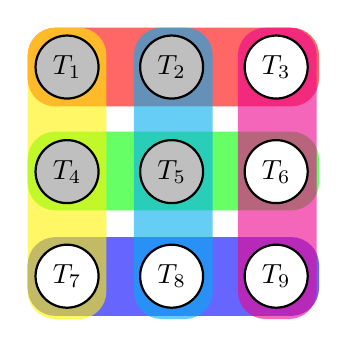
\begin{tikzpicture}[
    semithick,
    ]
    \tikzstyle{every state}=[ draw = black, thick, fill = white, minimum size = 8mm ]
    \draw[fill=red,draw=none,rounded corners=10pt, fill opacity = 0.6] (-0.5,0.5)    rectangle (3.2,-0.5);
    \draw[fill=green,draw=none,rounded corners=10pt, fill opacity = 0.6] (-0.5,-0.82)    rectangle (3.2,-1.82);
    \draw[fill=blue,draw=none,rounded corners=10pt, fill opacity = 0.6] (-0.5,-2.16)    rectangle (3.2,-3.16);
    \draw[fill=yellow,draw=none,rounded corners=10pt, fill opacity = 0.6] (-0.5,0.5)    rectangle (0.5,-3.2);
    \draw[fill=cyan,draw=none,rounded corners=10pt, fill opacity = 0.6] (0.85,0.5)    rectangle (1.85,-3.2);
    \draw[fill=magenta,draw=none,rounded corners=10pt, fill opacity = 0.6] (2.17,0.5)    rectangle (3.17,-3.2);
    \node[state, fill=lightgray] (T1) at (0,0){$T_1$};
    \node[state, fill=lightgray] (T2) [right=0.5cm of T1] {$T_2$}; 
    \node[state] (T3) [right=0.5cm of T2] {$T_3$}; 
    \node[state, fill=lightgray] (T4) [below=0.5cm of T1] {$T_4$};
    \node[state, fill=lightgray] (T5) [right=0.5cm of T4] {$T_5$}; 
    \node[state] (T6) [right=0.5cm of T5] {$T_6$}; 
    \node[state] (T7) [below=0.5cm of T4] {$T_7$};
    \node[state] (T8) [right=0.5cm of T7] {$T_8$}; 
    \node[state] (T9) [right=0.5cm of T8] {$T_9$}; 
  \end{tikzpicture}%
}
\end{figure}
\end{column}
\begin{column}{0.6\textwidth}
          \justify
% Without a hypergraph, the same data is counted multiple times.\\
Hypergraph $\rightarrow$ Represent a data being used by different tasks \\
%~ One hyperedge for each data $D$ $\rightarrow$ Includes all the vertices corresponding to tasks using $D$ $\rightarrow$
Accurately represent data shares
\end{column}
\end{columns}
	\setbeamercolor{block title}{bg=pink,fg=black}
	\begin{block}{Strategy}
	\begin{enumerate}
		\item Decompose the set of tasks into several subsets of similar size while minimizing the number of common data among subsets
		\item Each subset is allocated to a GPU
		\item Use the \emph{Ready} strategy
		\item Dynamic load balancing using task stealing
	\end{enumerate}
	\end{block}
\end{frame}

%~ %% ---------------------------------------------------------------------------
\subsection{Data-Aware Reactive Task Scheduling: DARTS}
%~ \begin{frame}{Data-Aware Reactive Task Scheduling: DARTS}
	%~ \begin{itemize}
		%~ \item \emph{Consider data movement before task allocation}
		%~ \item \example{Perform as many tasks as possible with
	%~ the data at hand} 
	%~ \end{itemize}
%~ \begin{figure}[tb]
%~ \definecolor{blue}{rgb}{0.38, 0.51, 0.71} %glaucous, 97,130,181, #6182B5
%~ \definecolor{darkblue}{RGB}{17, 42, 60} % 112A3C
%~ \definecolor{red}{RGB}{175, 49, 39} % AF3127
%~ \definecolor{lightred}{RGB}{220, 100, 100} % AF3127
%~ \definecolor{otherred}{RGB}{171,78,78}
%~ \definecolor{orange}{RGB}{237, 126, 75} 
%~ \definecolor{green}{RGB}{104, 174, 89} 
%~ \definecolor{palegreen}{RGB}{197, 184, 104} 

%~ \definecolor{yellow}{RGB}{250, 199, 70} % FAC764
%~ \definecolor{brokenwhite}{RGB}{218, 192, 166} % DAC0A6
%~ \definecolor{brokengrey}{rgb}{0.77, 0.76, 0.82} % {196,194,209}, C4C2D1

  %~ \scalebox{0.672}{
  %~ \begin{tikzpicture}[
    %~ semithick,
    %~ ]
    %~ \tikzstyle{every state}=[ draw = black, thick, fill = white, minimum size = 8mm ]
	

	%~ \node[state] (1) at (0, 0){};
	%~ \onslide<1> { \node[state] (2) [right=0.5cm of 1] {}; }
	%~ \node[state] (3) [right=0.5cm of 2] {};
	%~ \onslide<1-5> { \node[state] (4) [right=0.5cm of 3] {}; }
	%~ \onslide<1-3> { \node[state] (5) at (0, -1){}; }
	%~ \node[state] (6) [right=0.5cm of 5] {};
	%~ \onslide<1-7> { \node[state] (7) [right=0.5cm of 6] {}; }
	%~ \node[state] (8) [right=0.5cm of 7] {};
	%~ \node[state] (9) at (0, -2){};
	%~ \onslide<1-2> { \node[state] (10) [right=0.5cm of 9] {}; }
	%~ \node[state] (11) [right=0.5cm of 10] {};
	%~ \onslide<1-6> { \node[state] (12) [right=0.5cm of 11] {}; }
	%~ \onslide<1-4> { \node[state] (13) at (0, -3){}; }
	%~ \node[state] (14) [right=0.5cm of 13] {};
	%~ \onslide<1-8> { \node[state] (15) [right=0.5cm of 14] {}; }
	%~ \node[state] (16) [right=0.5cm of 15] {};
	
	%~ \onslide<2-3> { \node[state, fill = red!50] (16) [left=4cm of 1] {GPU asking for a task}; }
	%~ \onslide<4-5> { \node[state, fill = green!50] (16) [left=4cm of 1] {GPU asking for a task}; }
	%~ \onslide<6-7> { \node[state, fill = red!50] (16) [left=4cm of 1] {GPU asking for a task}; }
	%~ \onslide<8-9> { \node[state, fill = green!50] (16) [left=4cm of 1] {GPU asking for a task}; }
		
	%~ \node[state] (D1) [above=0.9cm of 1] {$D_1$}; 
    %~ \onslide<1> { \node[state] (D2) [above=0.9cm of 2] {$D_2$}; }
    %~ \node[state] (D3) [above=0.9cm of 3] {$D_3$}; 
    %~ \node[state] (D4) [above=0.9cm of 4] {$D_4$}; 
    %~ \onslide<1> { \node[state] (D5) [left=0.9cm of 1] {$D_5$}; }
    %~ \node[state] (D6) [left=0.9cm of 5] {$D_6$}; 
    %~ \onslide<1-2> { \node[state] (D7) [left=0.9cm of 9] {$D_7$}; }
    %~ \node[state] (D8) [left=0.9cm of 13] {$D_8$}; 
    
    %~ \onslide<2-> { \node[state, fill = red!50] (2) [right=0.5cm of 1] {$1$}; \node[state, fill = red!50] (D2) [above=0.9cm of 2] {$D_2$}; \node[state, fill = red!50] (D5) [left=0.9cm of 1] {$D_5$}; }
    %~ \onslide<3-> { \node[state, fill = red!50] (10) [right=0.5cm of 9] {$2$}; \node[state, fill = red!50] (D7) [left=0.9cm of 9] {$D_7$}; }
    %~ \onslide<4-> { \node[state, fill = green!50] (5) at (0, -1) {$1$}; \node[state, fill = green!50] (D1) [above=0.9cm of 1] {$D_1$}; \node[state, fill = green!50] (D6) [left=0.9cm of 5] {$D_6$};  }
    %~ \onslide<5-> { \node[state, fill = green!50] (13) at (0, -3){$2$}; \node[state, fill = green!50] (D8) [left=0.9cm of 13] {$D_8$}; }
    %~ \onslide<6-> { \node[state, fill = red!50] (4) [right=0.5cm of 3] {$3$}; \node[state, fill = red!50] (D4) [above=0.9cm of 4] {$D_4$};  }
    %~ \onslide<7-> { \node[state, fill=red!50] (12) [right=0.5cm of 11] {$4$}; }
    %~ \onslide<8-> { \node[state, fill = green!50] (7) [right=0.5cm of 6] {$3$};  \node[state, fill = green!50] (D3) [above=0.9cm of 3] {$D_3$}; }
    %~ \onslide<9-> { \node[state, fill = green!50] (15) [right=0.5cm of 14] {$4$}; }

%~ \end{tikzpicture}%
%~ }
%~ \end{figure}
%~ \end{frame}

%% ---------------------------------------------------------------------------
\begin{frame}{DARTS: Task flow}
%~ \begin{frame}{DARTS}
%~ \plannedTasks{k}: Task reserved for later allocation
%~ \pulledTasks{k}: Task popped from \plannedTasks{k} for execution on \GPU{k}

\begin{figure}[tb]
		\scalebox{0.79}{
		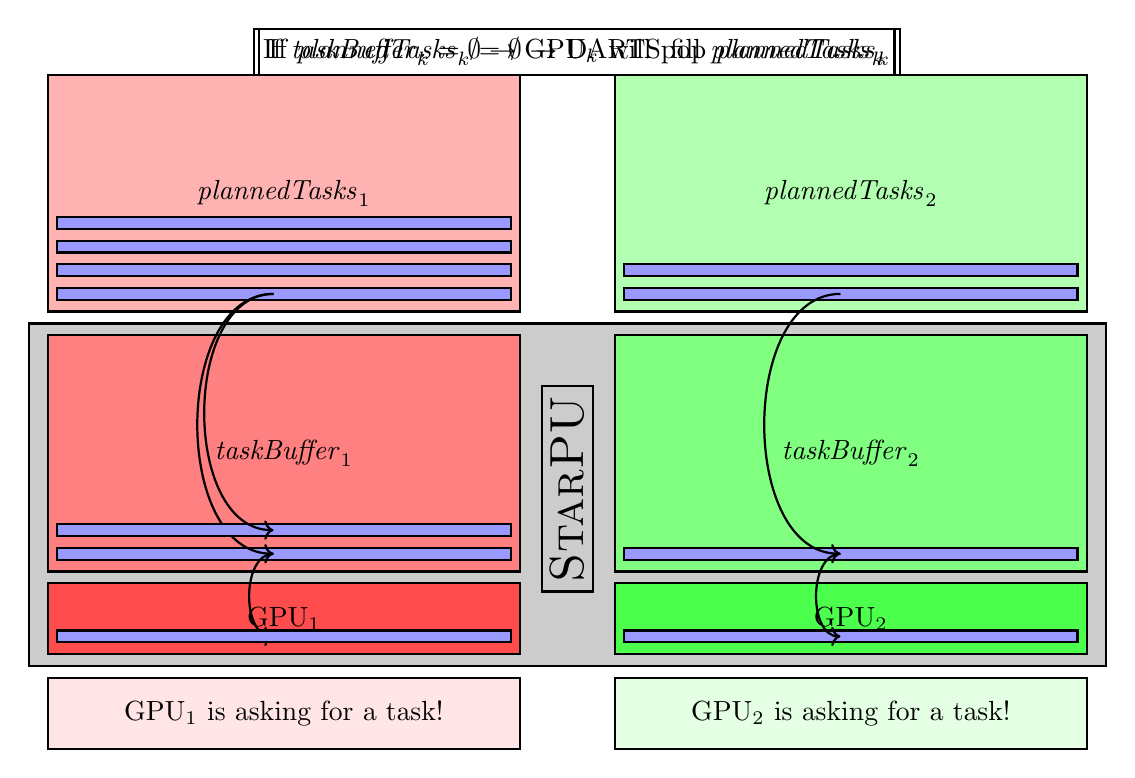
\begin{tikzpicture}[thick]
			\definecolor{orangegray}{RGB}{245, 191, 169}
			\def\x{1.2}
			\def\y{1.5}
			\draw[color=black, fill=gray!40] (-3.2*\x, 3.4*\y) rectangle (8.2*\x, 0.5*\y)  node[midway] {}; 
			\draw[color=black, fill=red!70] (-3*\x, 1.2*\y) rectangle (2*\x, 0.6*\y)  node[midway] {$\GPU{1}$}; 
			\draw[color=black, fill=red!50] (-3*\x, 3.3*\y) rectangle (2*\x, 1.3*\y)  node[midway] {$\pulledTasks{1}$}; 
			\draw[color=black, fill=red!30] (-3*\x, 5.5*\y) rectangle (2*\x, 3.5*\y)  node[midway] {$\plannedTasks{1}$}; 
			
			\draw[color=black, fill=green!70] (3*\x, 1.2*\y) rectangle (8*\x, 0.6*\y)  node[midway] {$\GPU{2}$}; 
			\draw[color=black, fill=green!50] (3*\x, 3.3*\y) rectangle (8*\x, 1.3*\y)  node[midway] {$\pulledTasks{2}$}; 
			\draw[color=black, fill=green!30] (3*\x, 5.5*\y) rectangle (8*\x, 3.5*\y)  node[midway] {$\plannedTasks{2}$}; 
						
			\node[draw, rotate=90] at (3, 3) {\LARGE $\starpu$};
			
			%~ \onslide<1-1> { \node[draw] at (0.6*\x, 5.7*\y) {$\plannedTasks{k}$: Task reserved for later allocation}; }
			%~ \onslide<1-1> { \node[draw] at (3.6*\x, 5.7*\y) {$\pulledTasks{k}$: Task popped for execution on $\GPU{k}$}; }
			
			\onslide<2-4> { \node[draw] at (2.6*\x, 5.7*\y) {If $\plannedTasks{k} = \emptyset \rightarrow$ DARTS fill $\plannedTasks{k}$}; }
			\onslide<5-6> { \node[draw] at (2.6*\x, 5.7*\y) {If $\pulledTasks{k} = \emptyset \rightarrow \GPU{k}$ will pop $\plannedTasks{k}$}; }
			
			\onslide<1-8> { \draw[color=black, fill=red!10] (-3*\x, 0.4*\y) rectangle (2*\x, -0.2*\y)  node[midway] {$\GPU{1}$ is asking for a task!}; }
			\onslide<9-12> { \draw[color=black, fill=green!10] (3*\x, 0.4*\y) rectangle (8*\x, -0.2*\y)  node[midway] {$\GPU{2}$ is asking for a task!}; }
			%~ \onslide<12-12> { \draw[color=black, fill=red!10] (-3*\x, 0.4*\y) rectangle (2*\x, -0.2*\y)  node[midway] {$\GPU{1}$ is asking for a task!}; }
			
			\onslide<2-> { \draw[color=black, fill=blue!40] (-2.9*\x, 3.7*\y) rectangle (1.9*\x, 3.6*\y)  node[midway] (1) {}; }
			\onslide<3-> { \draw[color=black, fill=blue!40] (-2.9*\x, 3.9*\y) rectangle (1.9*\x, 3.8*\y)  node[midway] (2) {}; }
			\onslide<4-6> { \draw[color=black, fill=blue!40] (-2.9*\x, 4.1*\y) rectangle (1.9*\x, 4.0*\y)  node[midway] (3) {}; }
			\onslide<5-5> { \draw[color=black, fill=blue!40] (-2.9*\x, 4.3*\y) rectangle (1.9*\x, 4.2*\y)  node[midway] (4) {}; } 
			 			 
			\onslide<6-> { \draw[color=black, fill=blue!40] (-2.9*\x, 1.5*\y) rectangle (1.9*\x, 1.4*\y)  node[midway] (5) {}; }
			
			%~ \onslide<6-6> { \path[every node/.style={font=\sffamily\small}] (1) edge[bend right=90] node [left] {} (5); }
			\onslide<6-6> { \draw[->] (1) edge[bend right=90] node [left] {} (5); }
			
			\onslide<7-7> { \draw[color=black, fill=blue!40] (-2.9*\x, 1.7*\y) rectangle (1.9*\x, 1.6*\y) node[midway] (6) {}; }
			
			%~ \onslide<7-7> { \path[every node/.style={font=\sffamily\small}] (1) edge[bend right=90] node [left] {} (6); }
			\onslide<7-7> { \draw[->] (1) edge[bend right=90] node [left] {} (6); }
			
			\onslide<8-> { \draw[color=black, fill=blue!40] (-2.9*\x, 0.8*\y) rectangle (1.9*\x, 0.7*\y) node[midway] (7) {}; }
			
			%~ \onslide<8-8> { \path[every node/.style={font=\sffamily\small}] (5) edge[bend right=90] node [left] {} (7); }
			\onslide<8-8> { \draw[->] (5) edge[bend right=90] node [left] {} (7); }
			
			\onslide<10-> { \draw[color=black, fill=blue!40] (3.1*\x, 3.7*\y) rectangle (7.9*\x, 3.6*\y)  node[midway] (8) {}; }
			\onslide<11-12> { \draw[color=black, fill=blue!40] (3.1*\x, 3.9*\y) rectangle (7.9*\x, 3.8*\y)  node[midway] (9) {}; }
			\onslide<12-13> { \draw[color=black, fill=blue!40] (3.1*\x, 1.5*\y) rectangle (7.9*\x, 1.4*\y)  node[midway] (10) {}; }
			\onslide<13-13> { \draw[color=black, fill=blue!40] (3.1*\x, 0.8*\y) rectangle (7.9*\x, 0.7*\y)  node[midway] (11) {}; }
			\onslide<13-> { \draw[color=black, fill=blue!40] (-2.9*\x, 0.8*\y) rectangle (1.9*\x, 0.7*\y)  node[midway] (12) {}; }
			
			\onslide<12-12> { \draw[->] (8) edge[bend right=90] node [left] {} (10); }
			\onslide<13-13> { \draw[->] (10) edge[bend right=90] node [left] {} (11); }
			
		\end{tikzpicture}
		}
\end{figure}
\end{frame}

%% ---------------------------------------------------------------------------
%~ \begin{frame}{Settings and buffers of task}
	%~ \begin{alertblock}{Initialization}
		%~ \begin{itemize}
			%~ \item Each GPU has a randomized data set: \Dtouse{k} (which initially contains all data)
			%~ \item Task set is randomized
		%~ \end{itemize}
	%~ \end{alertblock}
	%~ \begin{alertblock}{Each GPU has 2 buffers of task:}
		%~ \begin{enumerate}
			%~ \item \plannedTasks{k}: Task that have been reserved for a later allocation
			%~ \item \pulledTasks{k}: Task popped from \plannedTasks{k} for execution on \GPU{k}. Cannot be changed any more
		%~ \end{enumerate}
		%~ When \pulledTasks{k} is empty \GPU{k} will pop a task from \plannedTasks{k}.\\
		%~ When \plannedTasks{k} is empty, \GPU{k} call our algorithm to fill \plannedTasks{k}.
	%~ \end{alertblock}
%~ \end{frame}

%% ---------------------------------------------------------------------------
\begin{frame}{DARTS: Strategy}
	\begin{alertblock}{Intuition: consider data locality before task allocation}
		Perform as many tasks as possible with the data at hand
	\end{alertblock}
	
	When no more available tasks with data at hand:
	
	\begin{alertblock}{}
		%~ Everything is distributed. The scheduling is done by \GPU{k} when it needs new tasks.
		\begin{itemize}
			\item Find $D_{optimal}$ such that the number of tasks depending on $D_{optimal}$ and on other data already in memory is maximum
			%~ (if there is a tie: choose data with most total unprocessed task)
			\item $\plannedTasks{k} \gets$ set of unprocessed tasks depending only on $D_{optimal}$ and on other data already in memory 
			%~ \item Remove $\Dopt$ from \Dtouse{k}
			%~ \item If \Dopt does not allow to process at least one "free" task  -> Select a random unprocessed task \Treturned
		\end{itemize}
	\end{alertblock}
\end{frame}

%% ---------------------------------------------------------------------------
\begin{frame}{DARTS: Eviction and optimizations}
	\begin{alertblock}{Our eviction policy: LUF (Least Used in the Future)}
		% \begin{itemize}
			% \item Tasks in \plannedTasks{k} that have been reserved for a later allocation
			% \item Tasks in \pulledTasks{k}, that have been popped from \plannedTasks{k} for execution on \GPU{k}, and thus whose GPU placement cannot be changed any more
		% \end{itemize}
		\begin{enumerate}
			\item If possible, evict data not useful for any task in $\pulledTasks{k}$ and used by a minimal number of tasks in $\plannedTasks{k}$
			\item Otherwise, apply Belady's rule on tasks already allocated
			\item Update $\plannedTasks{k}$
		\end{enumerate}
	\end{alertblock}
	% \begin{alertblock}{Optimizations and improvements}
	\begin{alertblock}{Improvements}
		\begin{itemize}
			\item \threeinputs: Extension to deal with an heterogenous number of data per task
			%~ \item \bold{\OPTI}: We stop the search a soon as we find a data allowing to compute at least one task
			\item \OPTI: Reduce scheduling complexity by stopping earlier the search for $D_{opt}$
		\end{itemize}
	\end{alertblock}
\end{frame}

%% ---------------------------------------------------------------------------
\section{Experimental evaluation}
\subsection{Experimental settings}
\begin{frame}{Experimental settings}
    %~ \begin{columns}{}
        %~ \begin{column}{0.4\textwidth}
            %~ \justify
            %~ \begin{figure}
				%~ \centering
				%~ 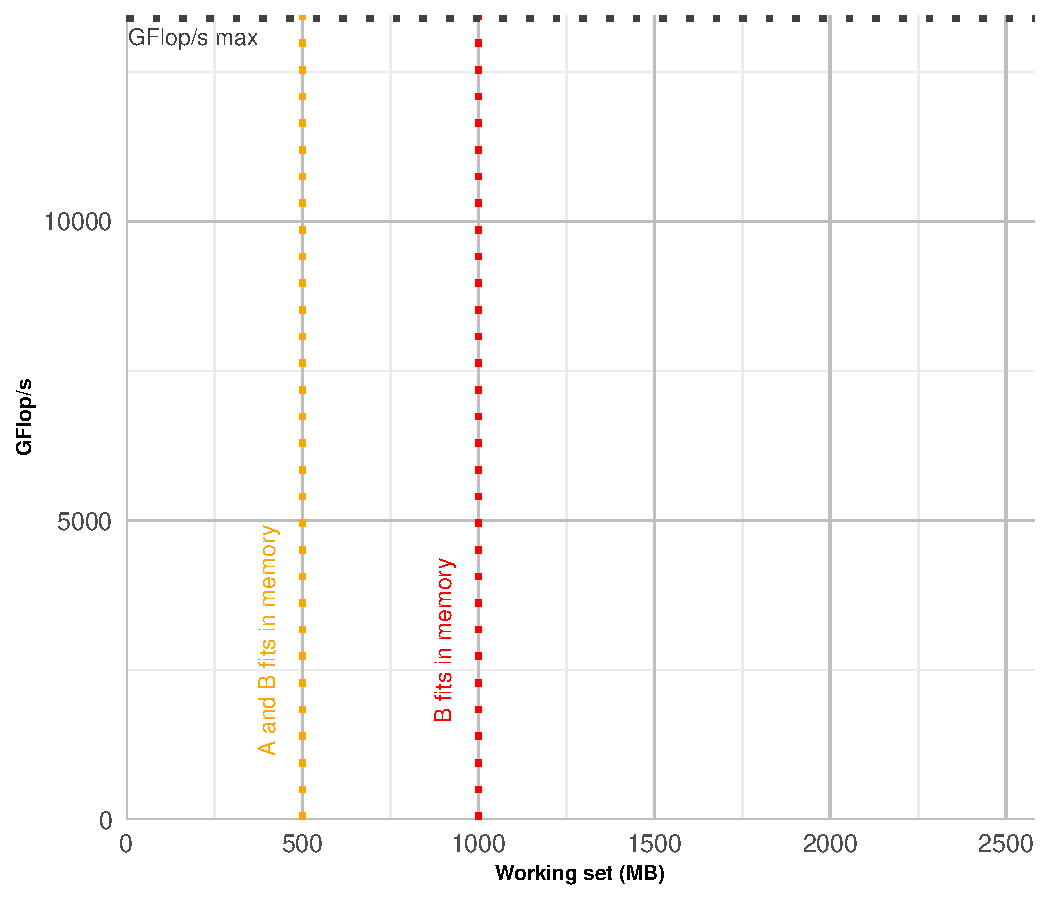
\includegraphics[scale=0.29]{Images/example_lines.pdf}
			%~ \end{figure}

        %~ \end{column}
        %~ \begin{column}{0.6\textwidth}
        \begin{block}{}
            \begin{itemize}
				\item Real Tesla V100 GPUs and simulations on Simgrid
				\item PCI bandwidth not limited ($12000\,MB/s$)
				\item GPU memory limited to $500\,MB$ $\rightarrow$ To better distinguish performance on small datasets
			\end{itemize}
		\end{block}
			\begin{block}{Applications}
			\begin{itemize}
				\item Tiled dense and sparse outer product 
				\item Tiled GeMM
				\item Tiled Cholesky decomposition (without dependencies)
			\end{itemize}
			\end{block}
        %~ \end{column}
    %~ \end{columns}
\end{frame}

%% ---------------------------------------------------------------------------
\subsection{Tiled dense outer product}
\begin{frame}{Tiled dense outer product with 2 real Tesla V100 GPUs}
    \begin{columns}{}
        \begin{column}{0.5\textwidth}
	\begin{figure}
		\center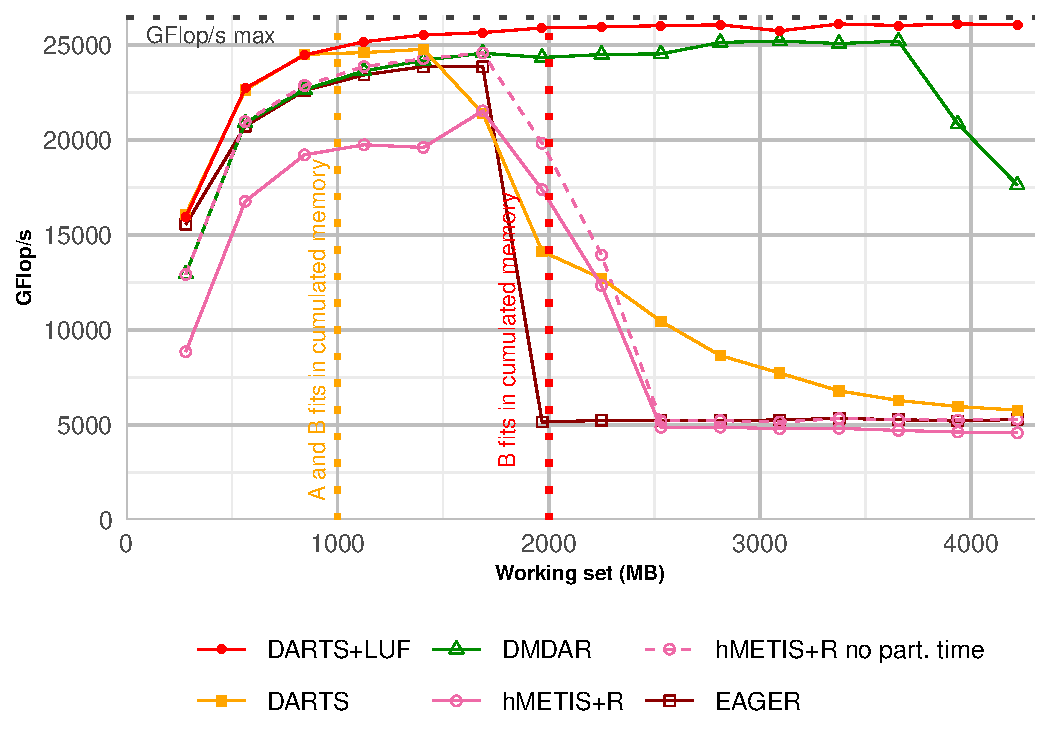
\includegraphics[scale = 0.3]{Images/GF_dynamic_data_aware_no_hfp_gemini-2-ipdps_2GPU.pdf}
	\end{figure}
	\end{column}
	%~ \begin{itemize}
		%~ \item EAGER, hMETIS \& DARTS: Pathological matrix size after the red line
		%~ \item DMDAR: Conflict between prefetch and eviction
	%~ \end{itemize}
%~ \end{frame}

%% ---------------------------------------------------------------------------
%~ \begin{frame}{Amount of data transfers on the dense outer product with 2 Tesla V100 GPUs}
    %~ \begin{columns}{}
        \begin{column}{0.5\textwidth}
	\begin{figure}
		%~ \center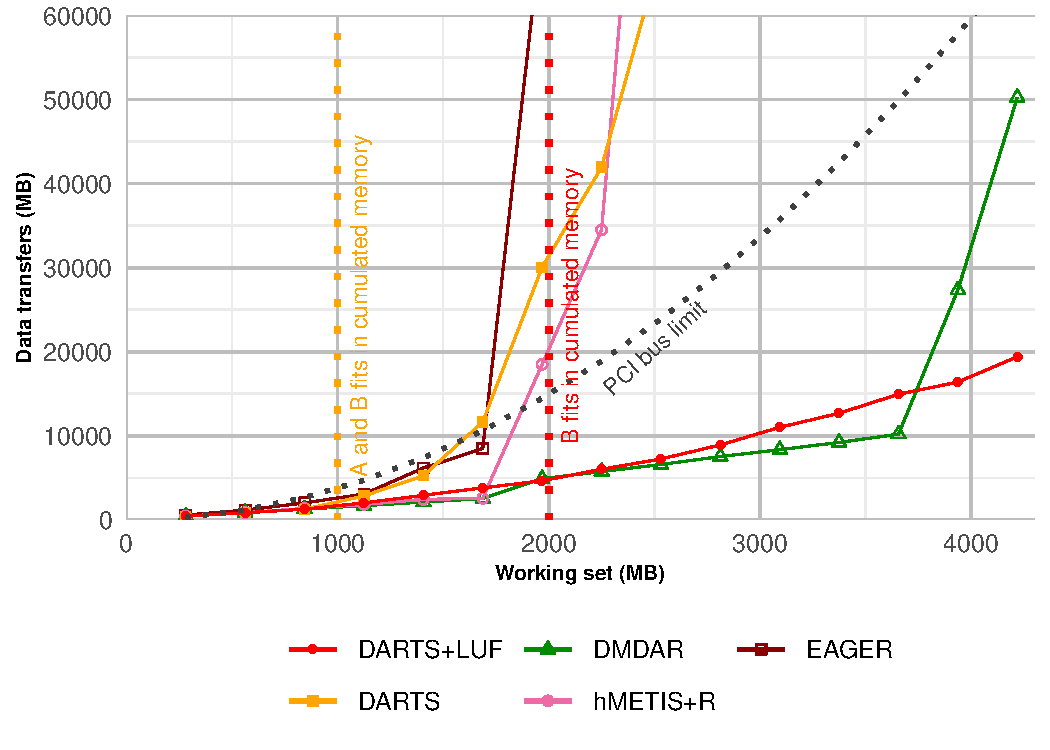
\includegraphics[scale = 0.25]{Images/DT_dynamic_data_aware_no_hfp_gemini-2-ipdps_2GPU.pdf}
		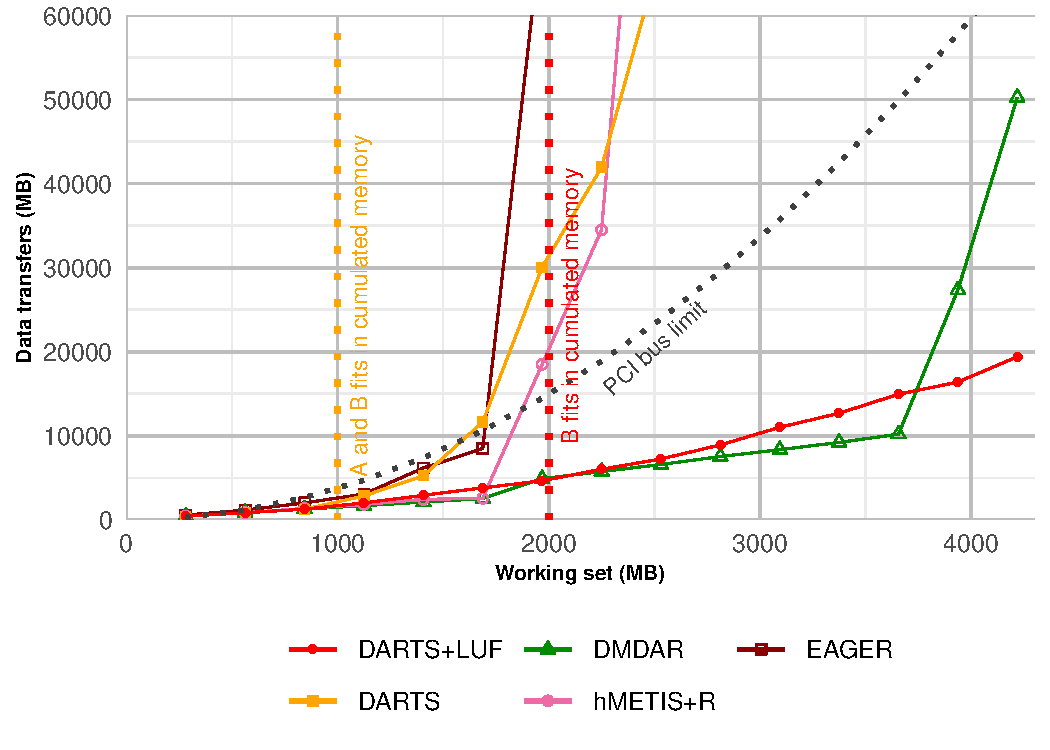
\includegraphics[scale = 0.3]{Images/DT_dynamic_data_aware_no_hfp_gemini-2-ipdps_2GPU.pdf}
		% \caption{Amount of data transfers on the 2D matrix multiplication in real with 2 Tesla V100 GPUs.}
	%~ \begin{itemize}
		%~ \item DARTS outperform DMDAR even with more data transfers $\rightarrow$ \emph{DARTS is better at 
		%~ overlapping communications and computations}
	%~ \end{itemize}
	\end{figure}
		\end{column}
		\end{columns}
	\begin{itemize}
		\item EAGER, hMETIS \& DARTS: Pathological matrix size after the red line
		\item DMDAR: Conflict between prefetch and eviction
		 \item DARTS+LUF outperforms DMDAR even with more data transfers $\rightarrow$ \emph{DARTS is better at 
		overlapping communications and computations}
	\end{itemize}
\end{frame}

%~ %% ---------------------------------------------------------------------------
%~ {
%~ \usebackgroundtemplate{}
%~ \subsection{3D matrix multiplication}
%~ \begin{frame}{3D matrix multiplication in simulation with the performance models of 4 Tesla V100 GPUs}
%~ % \begin{frame}{3D matrix multiplication in simulation with the performance models of 4 GPUs}
	%~ \begin{figure}
		%~ \center\includegraphics[scale = 0.45]{../Starpu/R/Courbes/Matrice3D/GF_dynamic_data_aware_no_hfp_gemini-1-fgcs_4GPU.pdf}
		%~ % \caption{Performance on the 3D matrix multiplication in simulation with the performance models of 4 Tesla V100 GPUs.}
	%~ \begin{itemize}
		%~ \item The \threeinputs improvement is crucial
	%~ \end{itemize}
	%~ \end{figure}
%~ \end{frame}
%~ }

%% ---------------------------------------------------------------------------
\subsection{Cholesky decomposition}
\begin{frame}{Cholesky decomposition with 4 real Tesla V100 GPUs}
    \begin{columns}{}
		\begin{column}{0.7\textwidth}
		\begin{figure}
			\center\includegraphics[scale = 0.45]{Images/GF_dynamic_data_aware_no_hfp_gemini-1-fgcs_4GPU.pdf}
		\end{figure}
		\end{column}
		\begin{column}{0.3\textwidth}
		\begin{itemize}
			\item \OPTI reduces scheduling time which improves performance
			\item DMDAR suffers from a large scheduling time
		\end{itemize}
		\end{column}
	\end{columns}
\end{frame}

%% ---------------------------------------------------------------------------
\section{Conclusion and future work}
\begin{frame}{Conclusion and future work}
\begin{block}{Limiting data movements is crucial to extract the most out of GPUs}
	Our contribution \MVRightarrow{}
	\emph{DARTS+LUF, focused on data locality}
\end{block}
\begin{exampleblock}{DARTS achieves very good performance because it:}
	%~ \example{Tested on 2D, 3D, sparse matrix multiplication and Cholesky decomposition}
	%~ \MVRightarrow{}
	%~ \emph{DARTS achieves very good performance because:}
		\begin{itemize}
			\item \textbf{Limits data transfers} thanks to the finding of an optimal data and the adapted eviction policy 
			\item \textbf{Overlaps} communication and computation by distributing transfers over time
			%~ \item Can be adapted to applications with \textbf{different number of inputs}
			\item Can be used with a \textbf{reduced complexity}
		\end{itemize}
\end{exampleblock}
	%~ \begin{block}{DARTS's limitations}
		%~ \begin{itemize}
		% \item Only manage a single node with several GPUs
		%~ \item Only manage a single MPI node
		% \item Does not consider tasks with dependencies
		%~ \item No dependencies
		%~ \end{itemize}
	%~ \end{block}
		
	\begin{exampleblock}{Areas for improvement}
		\begin{itemize}
		\item Improve computational complexity
		\item Take inter-GPU communications into account
		\item Consider tasks with dependencies
		\item Manage multiple MPI nodes
		\end{itemize}
	\end{exampleblock}
\end{frame}

% JOKER
\appendix{
%% ---------------------------------------------------------------------------
\begin{frame}[noframenumbering]{Dynamic Scheduling Strategies for Matrix Multiplication}
    \begin{figure}
        \centering
        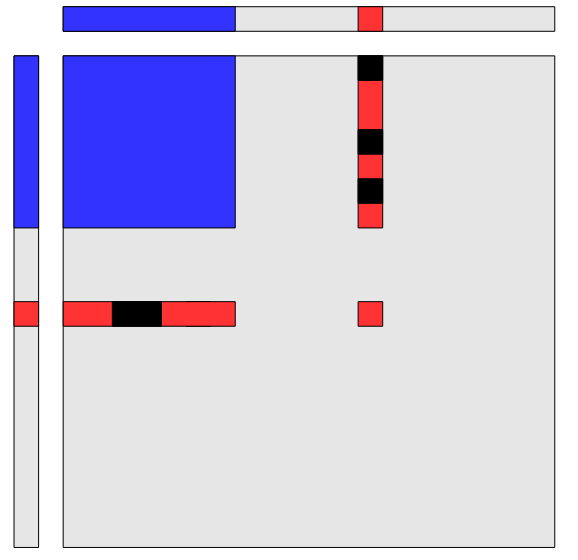
\includegraphics[scale=0.3]{Images/dynamic_outer_example.png}
        \source{Analysis of Dynamic Scheduling Strategies for Matrix Multiplication on Heterogeneous Platforms - Marchal - Beaumont}
    \end{figure}
\end{frame}

%% ---------------------------------------------------------------------------
\begin{frame}[noframenumbering]{Outer product with 4 Tesla V100 GPUs in real}
    \begin{figure}
        \centering
        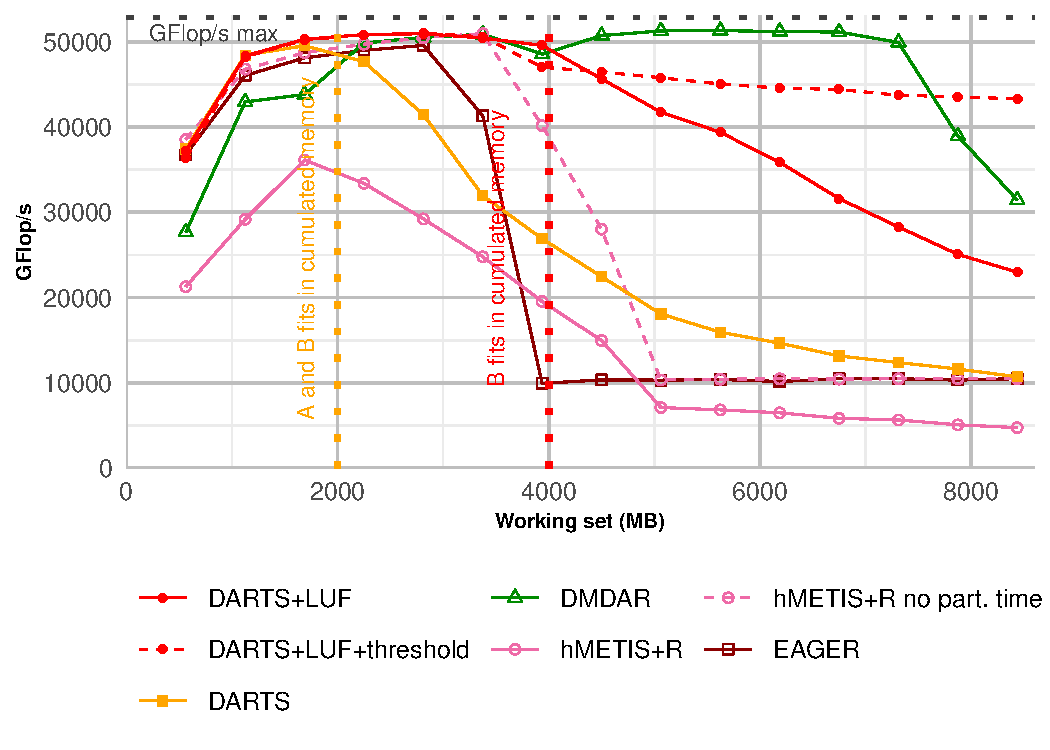
\includegraphics[scale=0.45]{Images/GF_dynamic_data_aware_no_hfp_gemini-2-ipdps_4GPU.pdf}
    \end{figure}
\end{frame}

%% ---------------------------------------------------------------------------
\begin{frame}[noframenumbering]{Tiled GeMM with 4 Tesla V100 GPUs in simulation}
    \begin{figure}
        \centering
        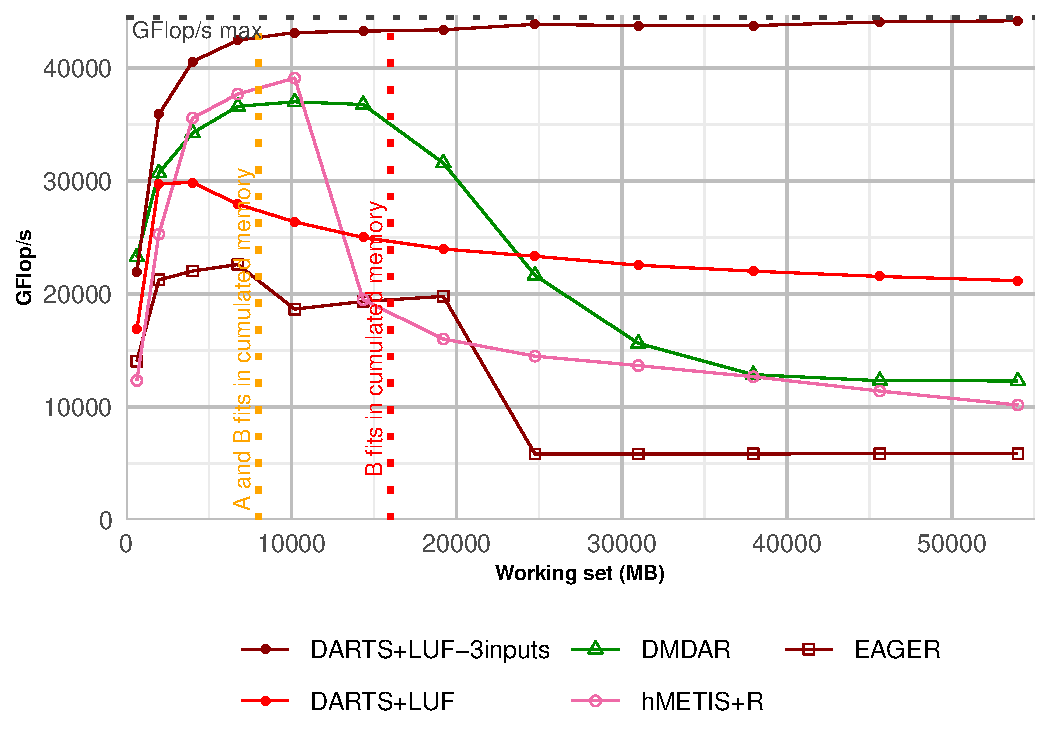
\includegraphics[scale=0.45]{Images/GF_dynamic_data_aware_no_hfp_gemini-1-fgcs_4GPU_M3D.pdf}
    \end{figure}
\end{frame}

%% ---------------------------------------------------------------------------
\begin{frame}[noframenumbering]{Sparse outer product without memory limitation (32GB by GPU) with 4 Tesla V100 GPUs}
    \begin{columns}{}
		\begin{column}{0.7\textwidth}
		\begin{figure}
			\center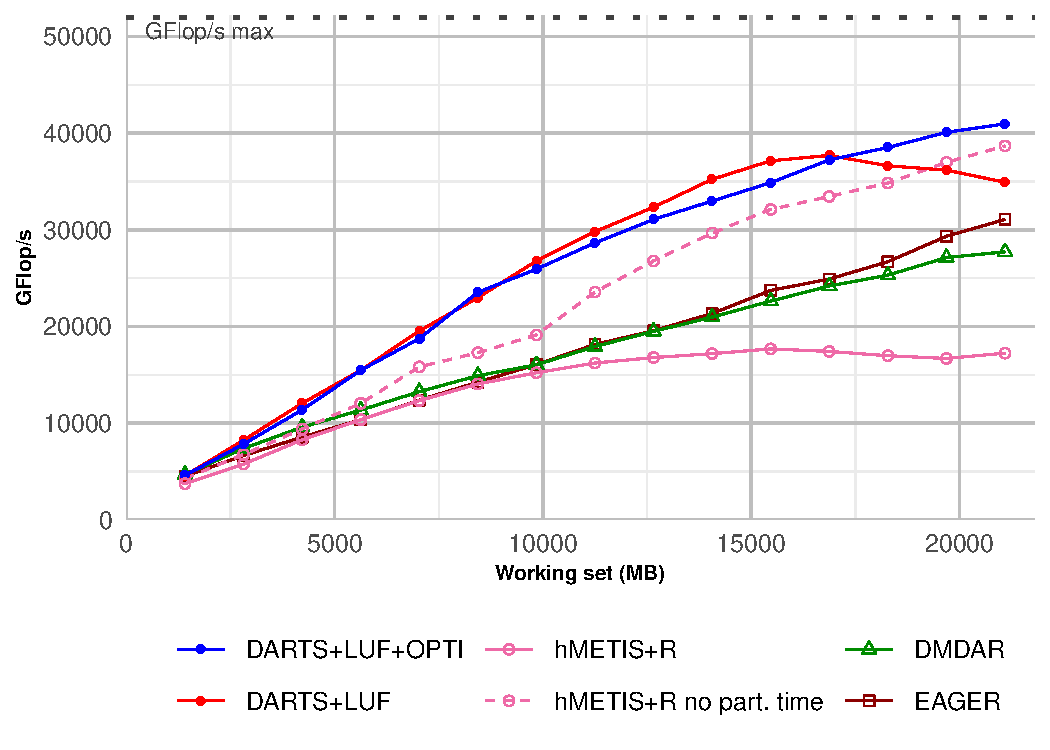
\includegraphics[scale = 0.45]{Images/GF_dynamic_data_aware_no_hfp_sparse_matrix_infinie_gemini-1-fgcs_4GPU.pdf}
		\end{figure}
		\end{column}
		\begin{column}{0.3\textwidth}
		\begin{itemize}
			\item DARTS produces a \emph{processing order that best distributes transfers over time} 
			\item hMETIS suffers from an important partitioning cost
		\end{itemize}
		\end{column}
	\end{columns}
\end{frame}
}

\end{document}
